\chapter{Introduction}
\section{Team}
\begin{itemize}
	\item Professor Richard Bucknall
	\item Mr Chris Greenough
	\item Mr Konrad Yearwood - Helpdesk email: k.yearwood@ucl.ac.uk
\end{itemize}
\section{Course Aim}
The aim of this course is to provide students with detailed knowledge and understanding of the design, performance and analysis of electrical power systems.

Students will increase their knowledge and understanding through face-to-face/synchronous lectures, asynchronous (including tutorials) tasks and a computer simulation workshop and demonstrate their learning through summative coursework and an examination.
\section{Student learning outcomes}
\begin{itemize}
	\item Appreciate the components that make up electrical power systems and understand the similarities and differences between large, medium and small scale power systems.
	\item Develop skills needed to be able to design electrical power systems including analytical and computer based methods.
	\item Understand the behaviour of steady-state, transient and faulted networks and appreciate how such behaviour influences design.
	\item Understand the benefits of electrical propulsion for different vehicle types be able to undertake designs.
	\item Appreciate future developments and applications in electrical power and electrical propulsion systems.
\end{itemize}
\section{Assessment}
\begin{itemize}
	\item Coursework - summative assessment exercise based around computer simulations
	\item Examination - two hour examination in January
\end{itemize}
\section{Textbooks}
Kirtley, James. \textit{Electric Power Principles: Sources, Conversion, Distribution and Use.} Wiley. 2020. ISBN: 9781119585305.t
\section{Softwares}
\begin{itemize}
	\item PSCAD
\end{itemize}
\chapter{The Electrical Line Diagram}
\section{Overview of electrical power systems}
\subsection{Basic electrical power system}
Most electrical power systems contain:
\begin{itemize}
	\item Generators to produce electrical energy (often coming from another store of energy e.g. chemical - oil, gas, coal)
	\item A means to transmit and distribute the electrical energy
	\item Loads that use the electrical energy for some purpose
\end{itemize}
\subsection{What is an electrical power system?}
\textbf{An electric power system} is a network or grid of electrical components that supply, transfer and use electric energy. Electrical power systems can be a:
\begin{itemize}
	\item Large grids covering a wide area e.g. a continent
	\item Medium grid covering a large area e.g. a country
	\item Small network covering a small area e.g. a ship
\end{itemize}
\section{Components of electrical power systems}
\subsection{Sources of electrical power include}
Generators (rotating types AC and DC):
\begin{itemize}
	\item Large AC generators e.g. \SI{25}{\kilo\volt} three-phase voltages
	\item Medium AC generators e.g. \SI{440}{\volt} three-phase voltages
	\item Small AC generators e.g. e.g. single-phase \SI{220}{\volt} voltages
\end{itemize}
Fuel cells:
\begin{itemize}
	\item DC output voltage (typically \SI{720}{\volt} DC)
\end{itemize}
Batteries (electro-chemical):
\begin{itemize}
	\item DC output voltage (usually multiples of \SI{12}{\volt})
\end{itemize}
Photo-voltaic (solar) cells:
\begin{itemize}
	\item DC output currents (usually mA/cell)
\end{itemize}
\subsection{Sources of DC electrical power \dots}
A fuel cell in a car. Photovoltaics used in a solar farm. Battery energy store. DC systems are increasing in their popularity due to wider use of batteries, solar cells and fuel cells in grids and electrical propulsion.
\subsection{Generators \dots single and multiphase AC}
AC generators:
\begin{itemize}
	\item Large AC generators e.g. \SI{25}{\kilo\volt} 3 phase
	\item Medium AC generators e.g. \SI{11}{\kilo\volt} or \SI{440}{\volt} 3 phase
	\item Small generators e.g. \SI{220}{\volt} single-phase voltage
\end{itemize}
\subsection{Transmission systems}
HVAC often three-wire and three-phase e.g. \SI{440}{\kilo\volt}, \SI{275}{\kilo\volt} and \SI{132}{\kilo\volt}.

HVDC often two-wire and bipolar e.g. +/- \SI{330}{\kilo\volt}.
\subsection{Distribution systems}
AC distribution:
\begin{itemize}
	\item \SI{11}{\kilo\volt}, \SI{440}{\volt} three-phase
	\item \SI{25}{\kilo\volt} single-phase (rail)
	\item \SI{240}{\volt} single-phase
\end{itemize}
DC distribution:
\begin{itemize}
	\item \SI{750}{\volt} (rail)
	\item \SI{110}{\volt} (emergency lighting)
\end{itemize}
\subsection{Loads}
Three-phase loads:
\begin{itemize}
	\item Induction motors to drive pumps, fans and compressors
	\item Propulsion drives
\end{itemize}
Single-phase loads:
\begin{itemize}
	\item Lighting
	\item Heating
	\item Appliances e.g. domestic, electronics, small pumps
\end{itemize}
DC loads:
\begin{itemize}
	\item DC motors
	\item Lighting and heating
	\item Battery charging
\end{itemize}
\section{Representation by the electrical line diagram}
\subsection{Electrical system representation}
Electrical systems are commonly represented as one of the following:
\begin{itemize}
	\item Pictorial diagram
	\item Block diagram
	\item Wiring diagram
	\item Single line diagram
	\item Riser diagram
	\item Electrical floor plan
	\item Layout diagram
\end{itemize}
Of these the most useful to the \textit{electrical power engineer} is the \textbf{Single line diagram.}
\begin{figure}[H]
	\centering
	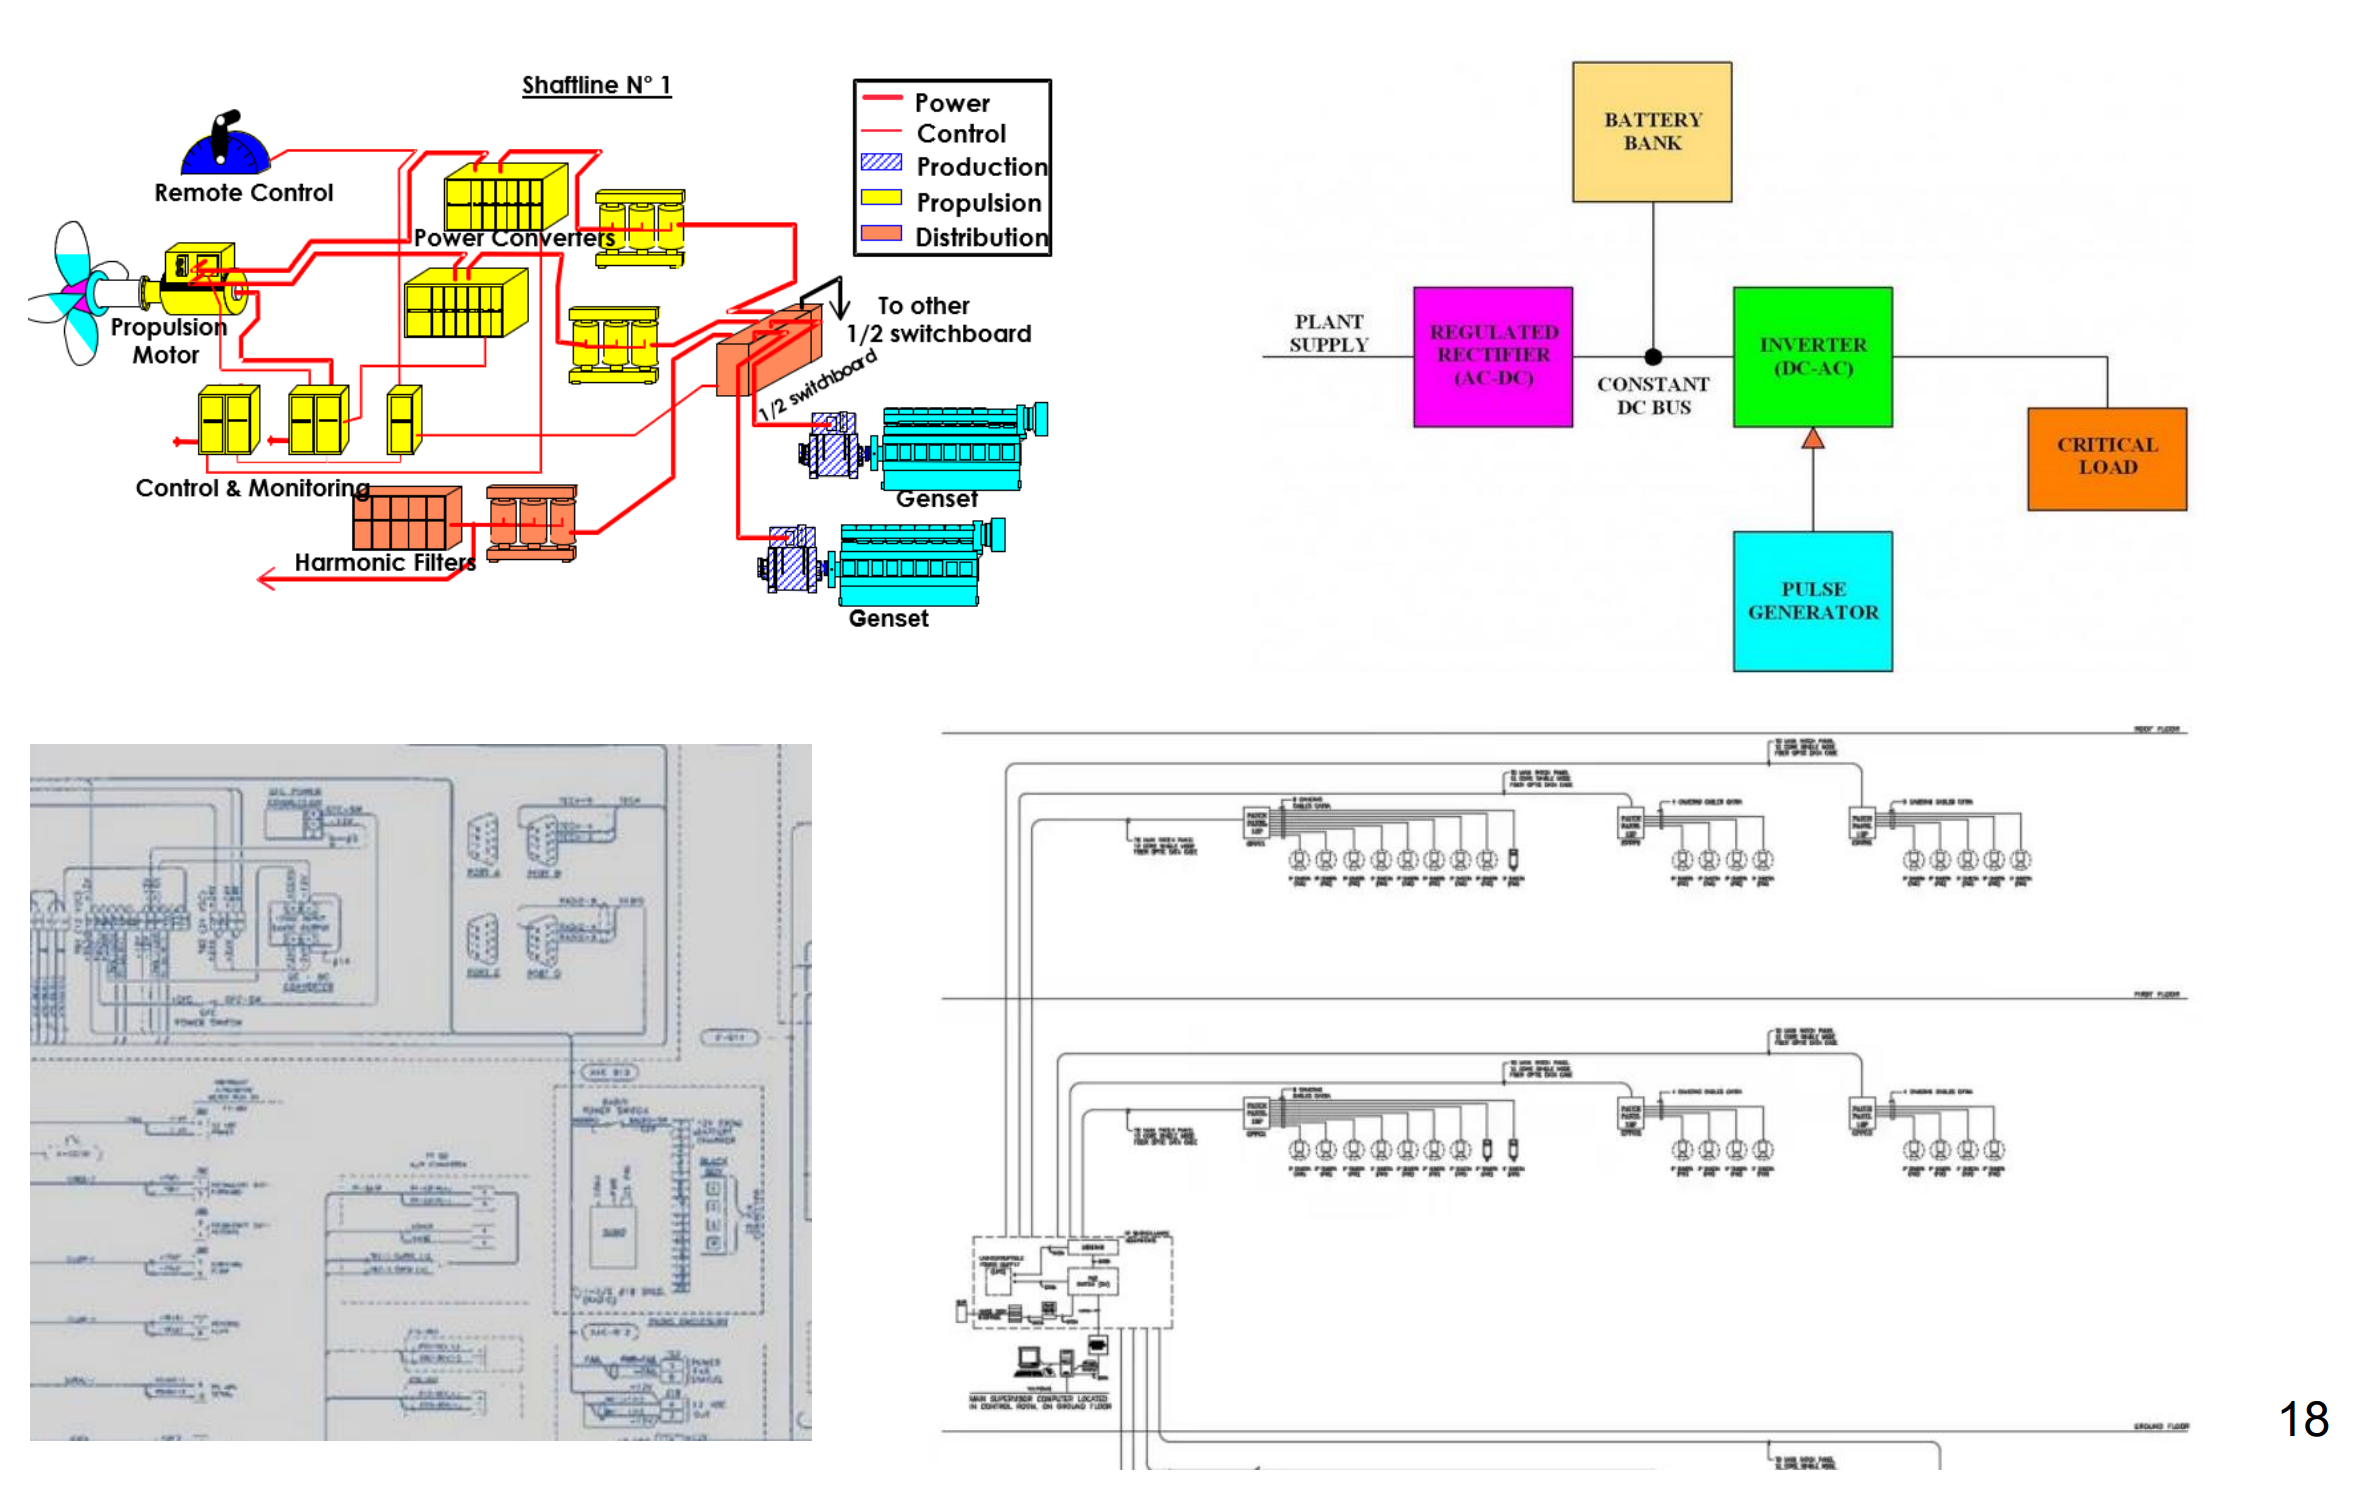
\includegraphics[width = \textwidth]{./img/figure1.png}
	\caption{Some types of electrical system representation.}
\end{figure}
\begin{figure}[H]
	\centering
	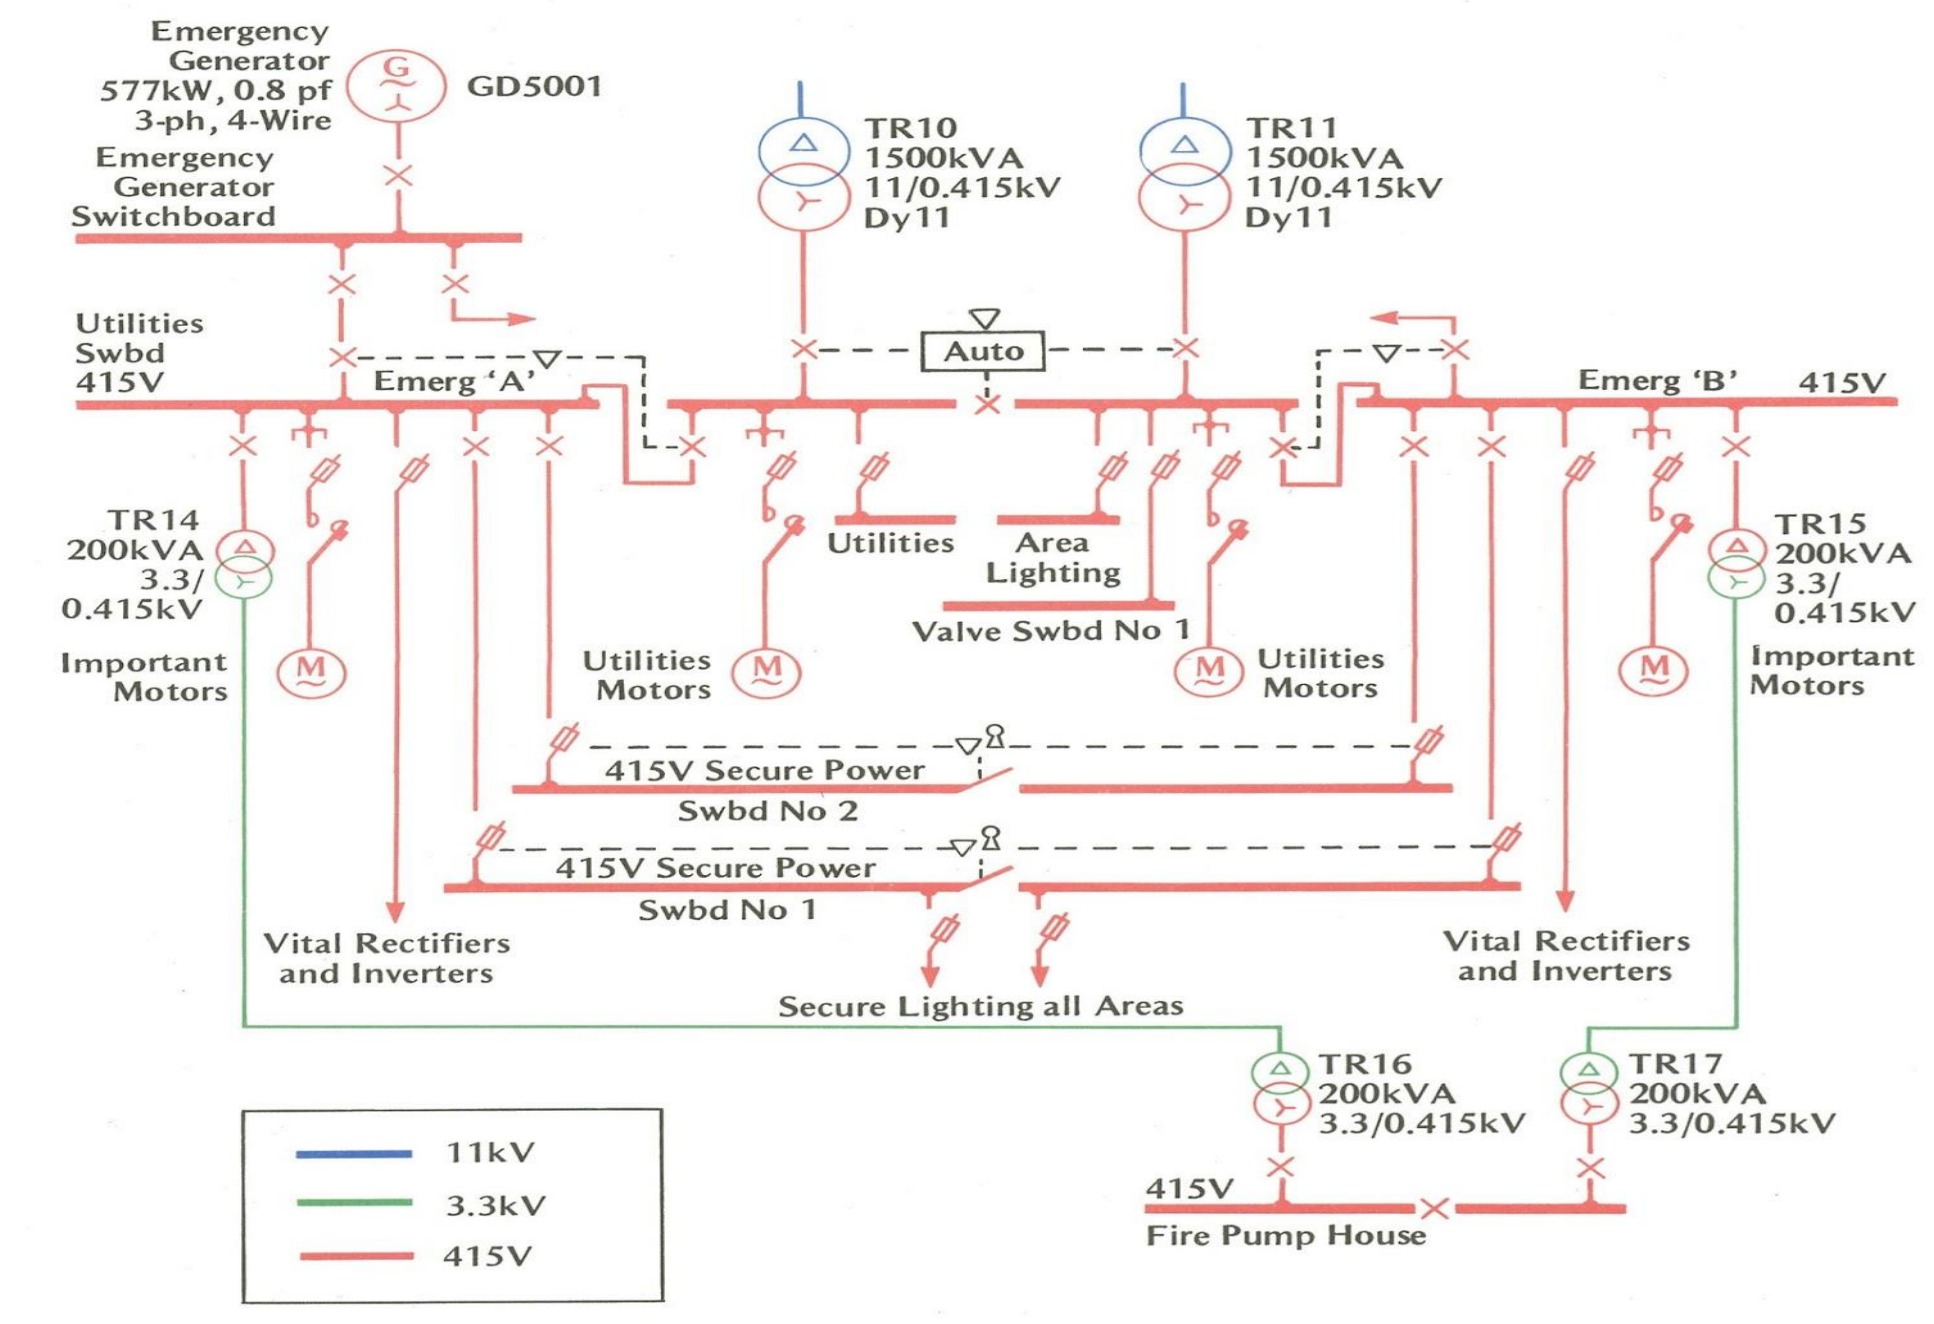
\includegraphics[width = \textwidth]{./img/figure2.png}
	\caption{Example of a `Single Line diagram'.}
\end{figure}
\subsection{Questions for you?}
\begin{enumerate}
	\item The number of separate switchboards shown? 14 (each thick line is a separate switchboard)
	\item Maximum current that will flow through the supply transformers? $I = \dfrac{\si{\kilo\volt\ampere}}{\si{\kilo\volt} \times \sqrt{3}}$, (root 3 due to 3-phase)
	\item How many different electrical sources supply the fire pump house? All three supplies can be connected to the fire pump house.
	      \begin{figure}[H]
		      \centering
		      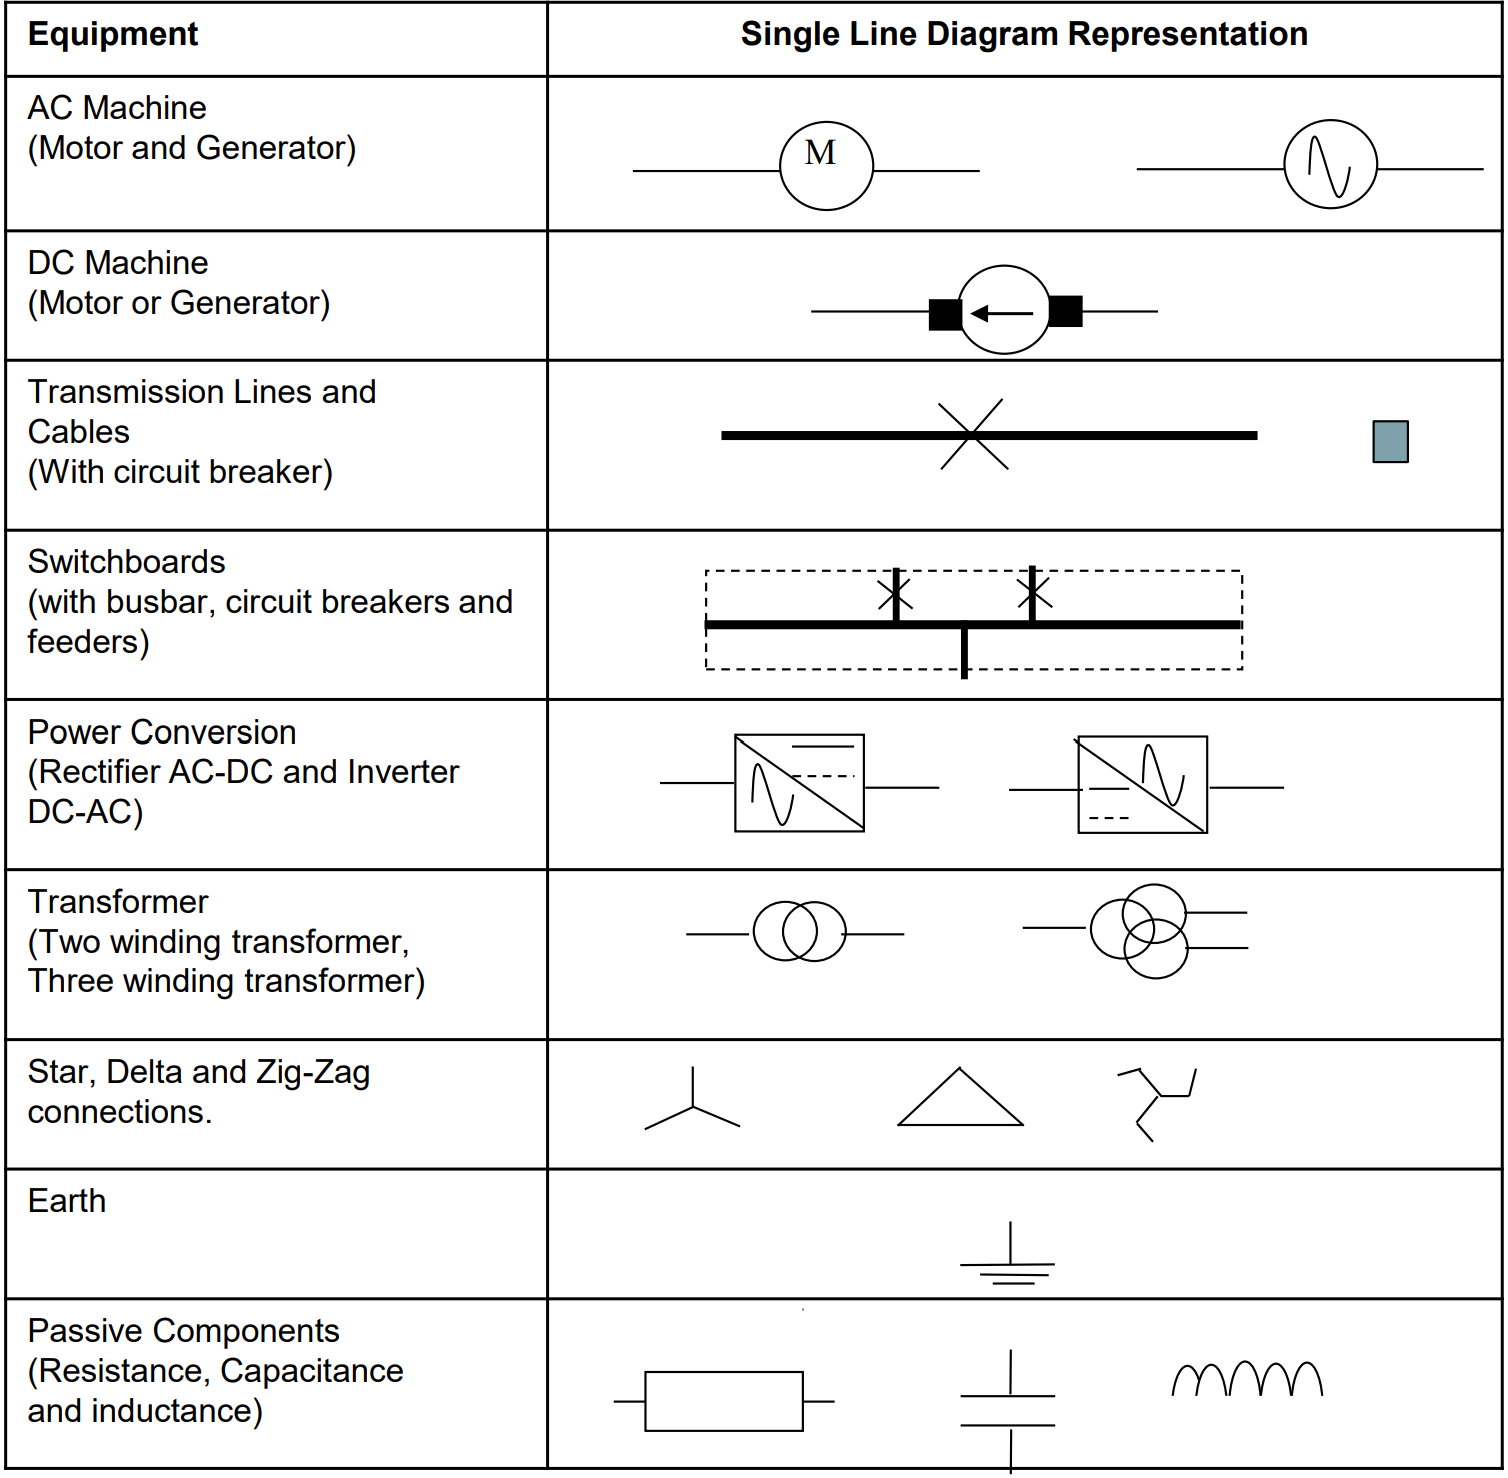
\includegraphics[width = \textwidth]{./img/figure3.png}
		      \caption{Symbols.}
	      \end{figure}
\end{enumerate}
\subsection{The `Single Line Diagram' (SLD)}
The `Single Line Diagram' (also known as the `One Line Diagram') represents an electrical power system using single lines regardless of number of cables being used. It can be used to represent:
\begin{itemize}
	\item Any type of electrical power system: DC, single-phase, three-phase or a mixed voltage electrical system.
	\item The interconnections between different electrical equipment including generators, switchboards, electrical distribution centres and loads.
	\item The types of electrical equipment and their main characteristics e.g. ratings of equipment such as voltage, power, power factor, and impedance.
	\item Emergency features such as reversionary modes, cross-connections and emergency generators. Sometimes these can be represented as single `dotted line' connections rather than the usual solid single line.
	\item Other details such as `earthing arrangements, arrangements of star/delta connections in three-phase systems and any autonomous operating systems such as circuit breakers.
\end{itemize}
\begin{figure}[H]
	\centering
	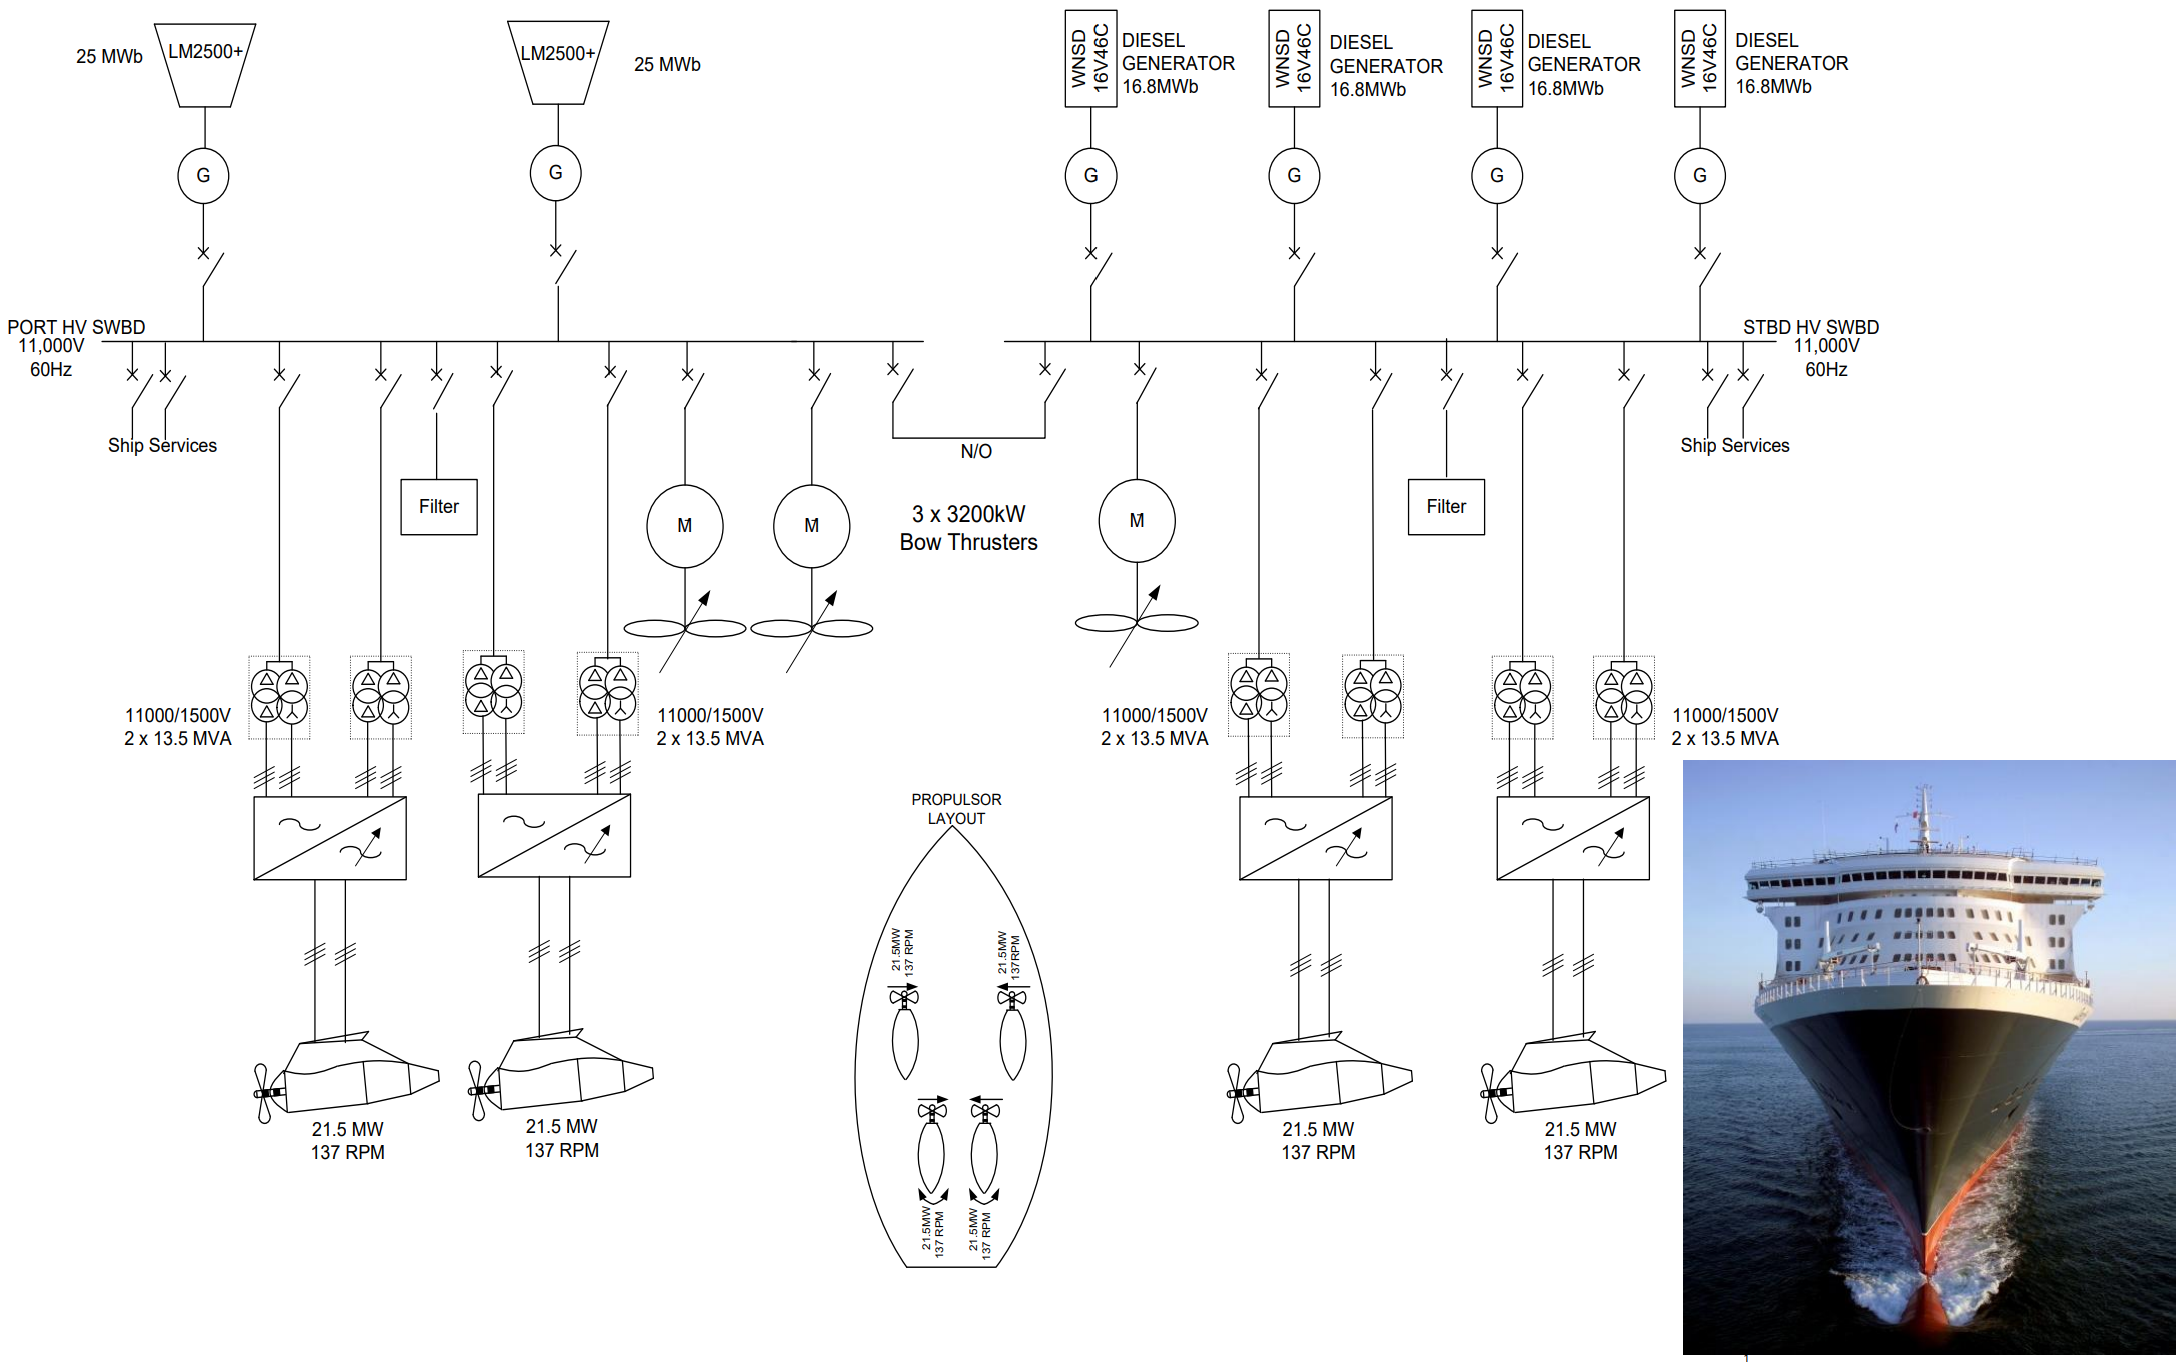
\includegraphics[width = \textwidth]{./img/figure4.png}
	\caption{Marine SLD.}
\end{figure}
\begin{figure}[H]
	\centering
	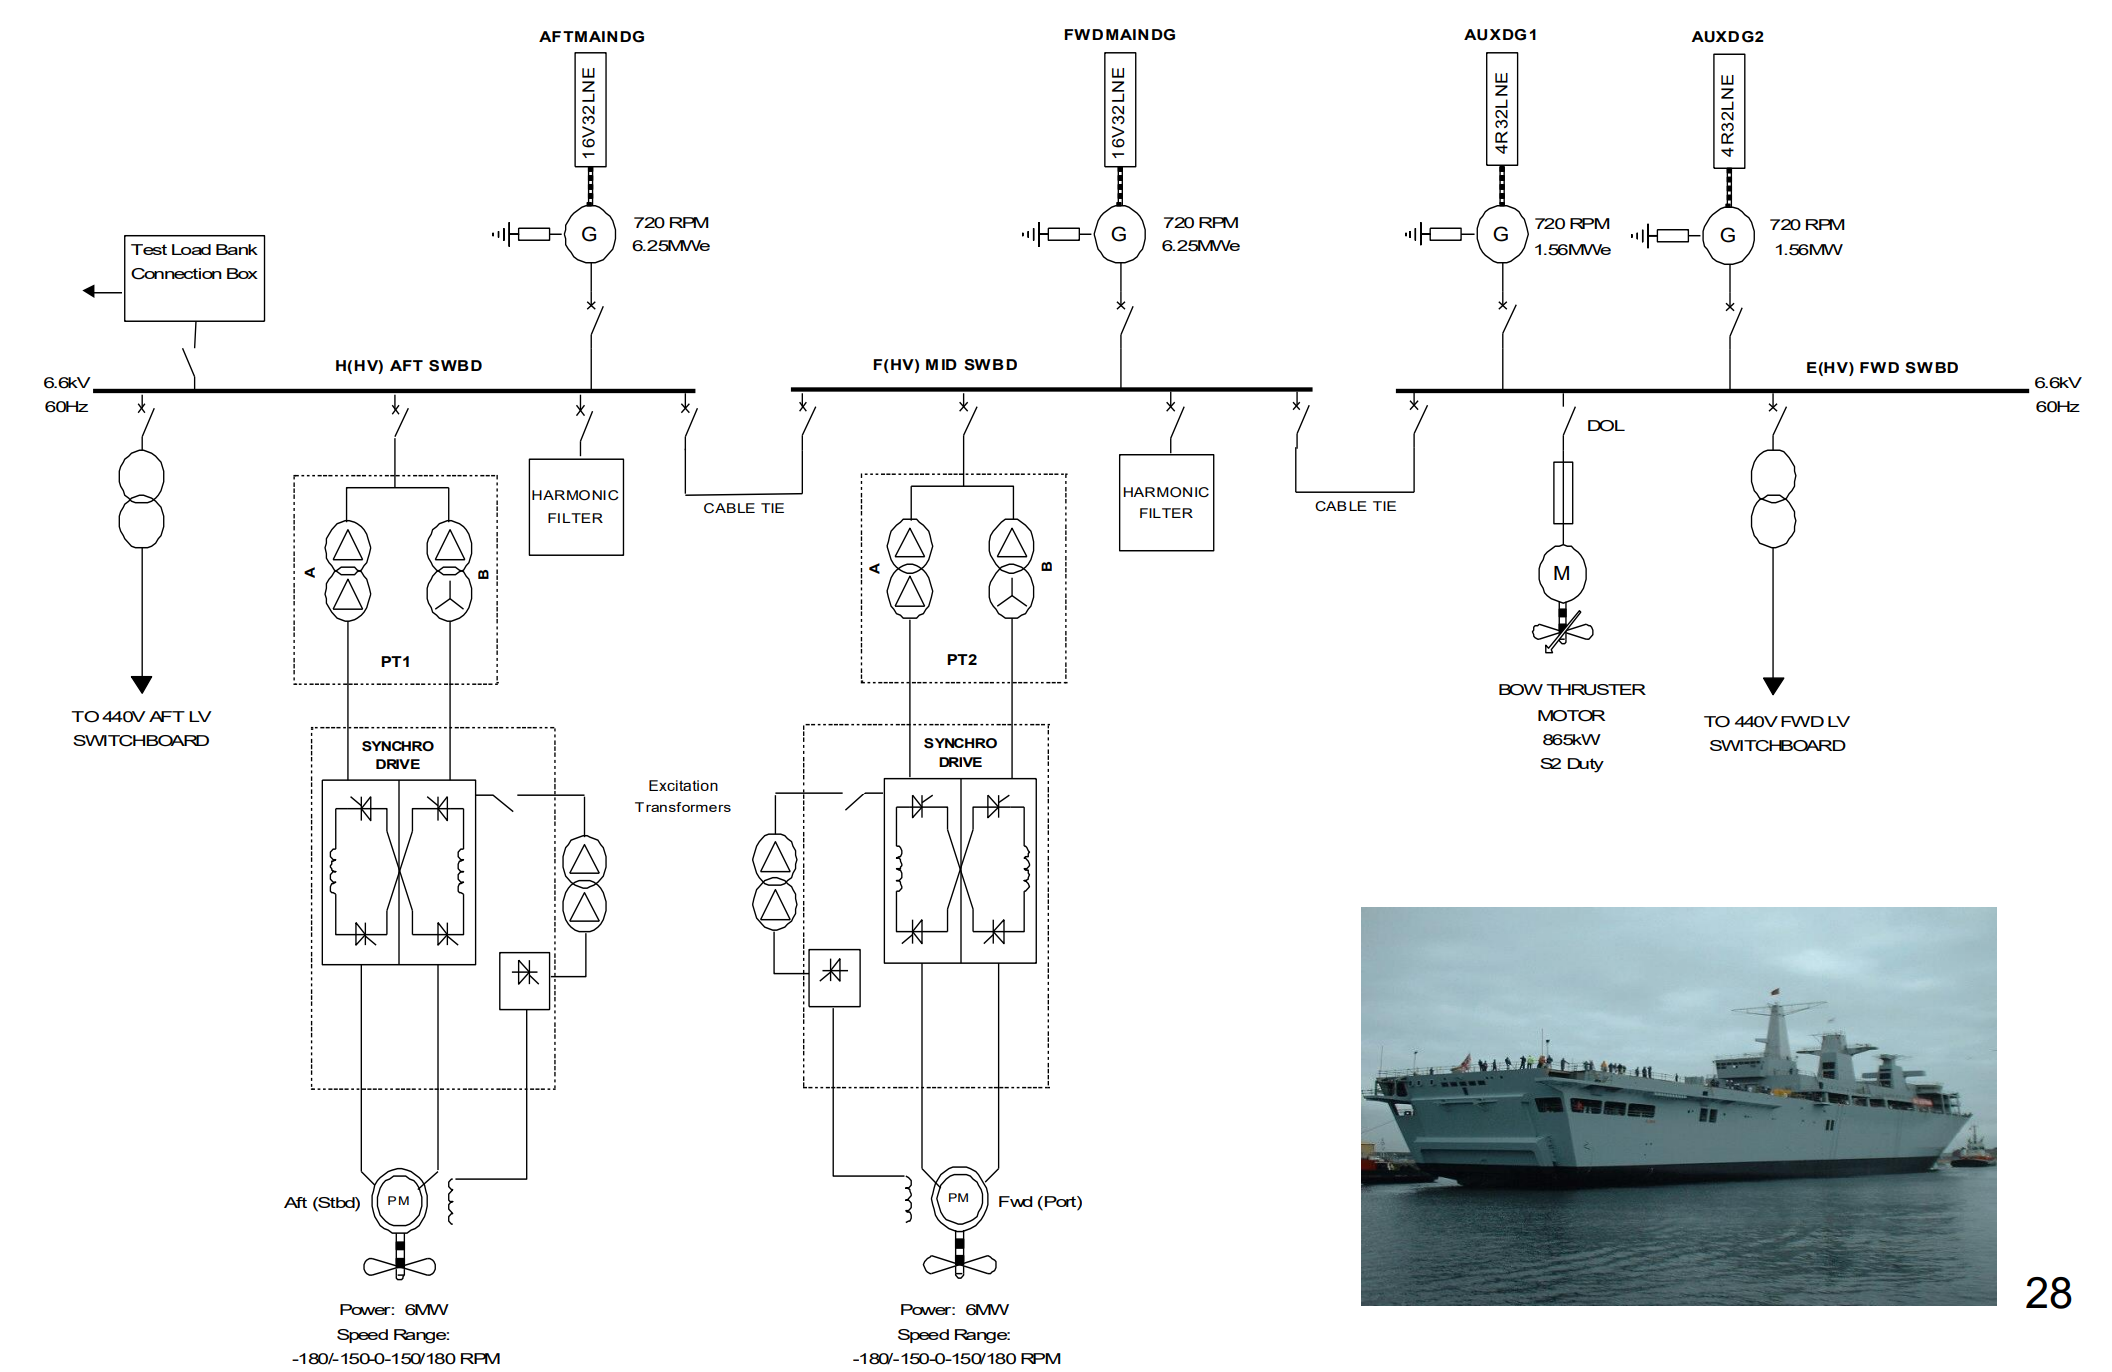
\includegraphics[width = \textwidth]{./img/figure5.png}
	\caption{Naval SLD.}
\end{figure}
\subsection{Some common features of SLDs}
\begin{itemize}
	\item Supplies (shore supplies, generators, incoming supply) are located at the top of the diagram
	\item The loads (motors, lighting, etc.) are located towards the bottom of the diagram.
	\item Switchboards are shown as thicker lines with interlocking switchgear being shown using dotted lines.
	\item Interconnections between equipment is a single-line representation regardless of number of phase (unless there is a good reason not to do so).
	\item Voltage, Frequency, Power, PF, revolutions, etc. are provided.
\end{itemize}
\subsection{Limitations of the electrical line diagram}
\begin{itemize}
	\item The `Single Line Electrical Diagram' is a very useful means of showing how electrical equipment is connected into a system using single lines (representing a three-phase system or some other electrical power system).
	\item It has very limited use when undertaking analysis. It is not an electrical circuit. To undertake analysis of electrical power systems then it is necessary to change the `Single Line Electrical Diagram' into an `Impedance Diagram'.
\end{itemize}













